\section{Příklad 4}
% Jako parametr zadejte skupinu (A-H)
\ctvrtyZadani{C}

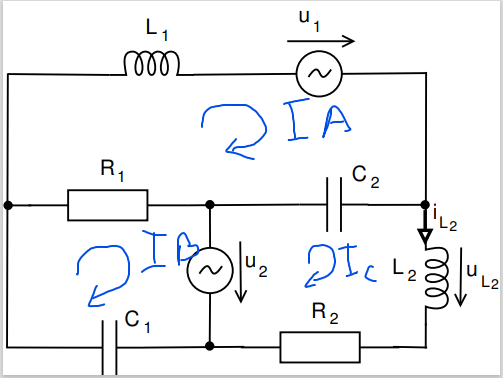
\includegraphics[scale=0.5,keepaspectratio]{picturesFor4Uloha/1.PNG} \\ 

Impedance pro cívku a kondenzátor:
\begin{align*}
	\omega &= 2\pi f \\
	Z_C &= \dfrac{-j}{\omega C}\\
	Z_L &=  j\omega L
\end{align*}

\begin{align*}
    I_A &:  U_{L1} + U_1 + U_{C2} + U_{R1} = 0 \\
    I_B &:  U_{R1} + U_2 + U_{C1} = 0 \\
    I_C &:  U_{C2} + U_{L2} + U_{R2} - U_2 = 0 \\
\end{align*}

\begin{align*}
    I_A &:  I_A * (Z_{L1} + Z_{C2} + R1) - I_B * R_1 - I_C * Z_{C2} = -U_1 \\
    I_B &:  -I_A * (R_1) + I_B * (R_1  + Z_{C1}) + 0 = -U_2 \\
    I_C &:  -I_A * Z_{C2} + 0 + I_C * (Z_{C2} + Z_{L2} + R2)  = U_2 \\
\end{align*}

Matice pro proudové smyčky: 

\begin{align*}
	\begin{pmatrix}
		Z_{L1}+Z_{C2}+R_1&-R_1&-Z_{C2}\\ 
		-R_1&R_1+Z_{C1}&0\\ 
		-Z_{C2}&0&Z_{C2}+R_2+Z_{L2}
	\end{pmatrix}
	*
	\begin{pmatrix}
		I_A\\ I_B\\ I_C
	\end{pmatrix}
	=
	\begin{pmatrix}
		-U_1\\ -U_2\\ U_2
	\end{pmatrix}
\end{align*}


\begin{align*}
	\omega &= 2\pi f\\
	Z_{C1} &= \dfrac{-j}{\omega C_1} \\
	Z_{C2} &= \dfrac{-j}{\omega C_2}\\
	Z_{L1} &=  j\omega L_1 \\
	Z_{L2} &=  j\omega L_2 \\
\end{align*}

\begin{align*}
	\begin{pmatrix}
		10 + 78.707j&-10&24.9655j\\ 
		-10&10 - 9.2264j&0\\ 
		24.9655j&0&13 + 8.0212j
	\end{pmatrix}
	*
	\begin{pmatrix}
		I_A\\ I_B\\ I_C
	\end{pmatrix}
	=
	\begin{pmatrix}
		-3\\ -4\\ 4
	\end{pmatrix}
\end{align*}

\begin{align*}
	I_A &= (-0.171241 + 0.035563j)\Am \\
	I_B &= (-0.3263 - 0.2655j)\Am \\
	I_C &= (0.419275 + 0.070155j)\Am
\end{align*}

\subsection{Výpočet}

\begin{quote}
    \centering
	$I_C = I_{L2}$ \\
	$U_{L2} = I_{L2} * Z_{L2}$ \\~\\
	\medskip
	$\varphi_{L_{2}} = arctan(\dfrac{imag(U_{L2})}{real(U_{L2})}) * \dfrac{\pi}{180} + \pi$ \\~\\
	\medskip
	$|U_{L2}| = \sqrt{real(U_{L2})^2 + imag(U_{L2})^2}$
\end{quote}

\newpage
\begin{quote}
    \centering
	$I_C = I_{L2} = (0.419275 + 0.070155j)\Am$ \\~\\
	\medskip
	$U_{L2} = (0.419275 + 0.070155j)\Am * 32.9867j = (-2.3142 + 13.8305j)\Vo$ \\~\\
	\medskip
	$\varphi_{L_{2}} = (arctan(\dfrac{13.8305}{-2.3142}) * \dfrac{\pi}{180} + \pi) * \dfrac{180}{\pi} = 178.59499^\circ$ \\~\\
	\medskip
	$|U_{L2}| = \sqrt{(-2.3142)^2 + 13.8305^2} = 14.02278\Vo = 14.023\Vo$
\end{quote}

